\documentclass[a4paper,12pt,ngerman,fleqn]{article}

    \renewcommand{\familydefault}{\sfdefault}
    \usepackage[a4paper, margin={0cm,0cm},twocolumn, layouthoffset=0pt]{geometry}
    
    \usepackage{tikz}
    \usepackage{framed}
    \usepackage{amsmath}
    \setlength{\mathindent}{0pt}
    \usepackage{amsfonts}
    \usepackage{amssymb}
    \usepackage{tabularx, colortbl}

    \usepackage{xcolor}
    \definecolor{accent}{HTML}{0eb7ac}

    \linespread{1}
    \vspace{1cm}
    \renewcommand{\arraystretch}{2}
    \arrayrulecolor{accent}
    \setlength\arrayrulewidth{1.5pt}
    \renewcommand{\baselinestretch}{0.8} 
    \newcommand{\mybox}[3]{
        \centering
        \begin{tabularx}{0.9\textwidth}{|X|}
            \rowcolor{accent}
            \rule{0pt}{20pt}
            \textcolor{white}{\textbf{#1}} \\
            \def\temp{#2}\ifx\temp\empty
                
            \else
                #2 \\ \hline
            \fi
            #3
            \\ \hline
        \end{tabularx}
    }

\begin{document}
    
    \setlength{\parindent}{0cm}

    \begin{tikzpicture} 
        \fill[accent, opacity=1] (0,0) rectangle (21,3);
        \fill[accent, opacity=0.8] (0,-2) rectangle (21,0);
        \fill[accent, opacity=1] (1.5,0.1)
            -- (2,-0.5)
            -- (2.5,0.1)
            -- cycle;
        \node[anchor=east,text=white] (why1) at (6.8,1.5) {\huge Neural Networks};
        \node[anchor=east,text=white] (why1) at (12.7,-1.2) {
            Neural networks are limited imitations of how our own brains work.
        };
    \end{tikzpicture}

    % LEFT SIDE OF SHEAT
    \begin{minipage}[t]{.51\textwidth}
        \vspace{1pt}
        \mybox
            {Visual Representation}
            {
                {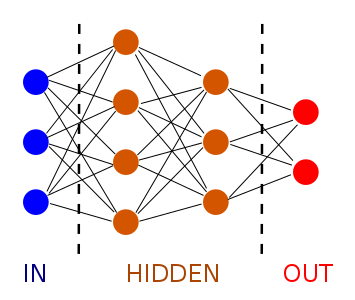
\includegraphics[width=0.6\textwidth, height=40mm]{Nn_00.png}}
            }
            {
                - Input and Output mandatory \\
                - Hidden is optional but recommanded \\
                - 0..N Hidden Layer possible \\
                - 0..N Neuron per each Hidden layer possible
            }
        \newline
        \newline
        \newline
        \mybox
            {Output Hypothesis calculation}
            {
                {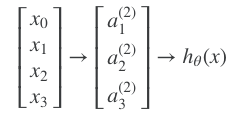
\includegraphics[width=0.65\textwidth, height=28mm]{NN_4Input_3hidden_1output.png}} \\
                {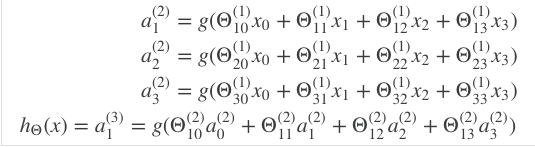
\includegraphics[width=0.85\textwidth, height=33mm]{values_each_activation_note.png}}
            }
            {
                - \(a_i^{(j)} = \text{"activation" of unit $i$ in layer $j$} \) \\
                - \(\Theta^{(j)} = \text{matrix of weights controlling function} \) \\
                \( \text{mapping from layer $j$ to layer $j+1$} \)
            }
        \newline
    \end{minipage}%
    \begin{minipage}[t]{.51\textwidth}
        \vspace{1pt}
        \mybox
            {Back propagation Algorithm}
            {}
            {
                Given training set \( \{ (x^{(1)}, y^{(1)}) ... x^{(m)}, y^{(m)} \) \\
                - Set \( \Delta^{(l)}_{i,j} := \) for all (L,i,j) \\
                For training example t=1 to m: \\
                - Set \( a^{(i)} := x^{(t)}\) \\
                - Perform forward propagation to compute \( a^{(l)} \text{for} I=2,3,...,L \) \\
                - Using \( y^{(t)} \), compute \( \delta^{(L)} = a^{(L)} - y^{(t)} \) \\
                - Compute \( \delta^{(L-1)},\delta^{(L-2)},...,\delta^{(2)} \) using \( \delta^{(l)} = ((\Theta^{(l)})^T \delta^{(l+1)}). * a^{(l)}. * (1-a^{(l)})\) \\
                - \( \Delta^{(l)}_{i,j} := \Delta^{(l)}_{i,j} + a^{(l)}_j\delta^{(l+1)}_i\) \\
                - \( D^{(l)}_{i,j} := \dfrac{1}{m} (\Delta^{(l)}_{i,j} + \rightthreetimes\Theta^{(l)}_{i,j}) \text{ if j} \neq 0\) \\
                - \( D^{(l)}_{i,j} := \dfrac{1}{m} \Delta^{(l)}_{i,j} \text{j=0} \) \\
                - The capital-delta matrix is used as an "accumulator" to add up our values as we go along and eventually compute our partial derivative.
            }
        \newline
    \end{minipage}

    \vspace{125.5pt}
    \fcolorbox{accent}{accent}{
    \begin{minipage}[t]{1\textwidth}
        \vspace{2pt}
        \center
        \textcolor{white}{\scriptsize \copyright 2018 - Machine Learning Collection 3/3}
        \vspace{2pt}
    \end{minipage}
    }
    
\end{document}